\subsection{Useful reading}

\begin{frame}
  \frametitle{Useful Reading (1)}
  \begin{columns}
    \column{0.7\textwidth}
    Essential Linux Device Drivers, April 2008
    \begin{itemize}
    \item \url{https://elinuxdd.com/}
    \item By Sreekrishnan Venkateswaran, an embedded IBM engineer
      with more than 10 years of experience
    \item Covers a wide range of topics not covered by LDD: serial
      drivers, input drivers, I2C, PCMCIA, PCI,
      USB, video drivers, audio drivers, block drivers, network
      drivers, Bluetooth, IrDA, MTD, drivers in user space, kernel
      debugging, etc.
    \item \emph{Probably the most wide ranging and complete Linux
          device driver book I've read} -- Alan Cox
    \end{itemize}
    \column{0.3\textwidth}
    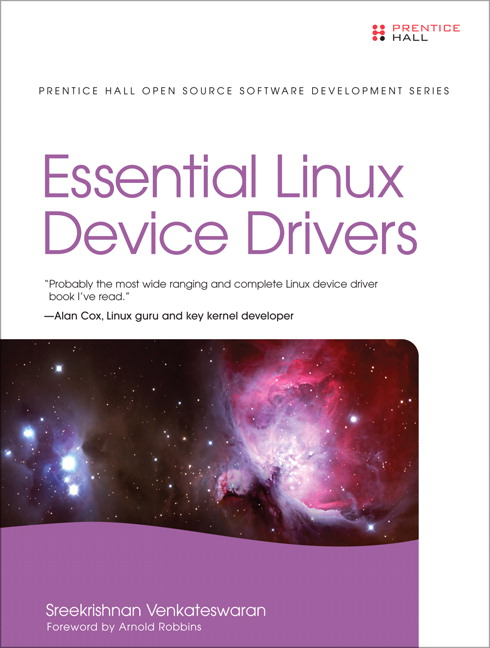
\includegraphics[width=\textwidth]{slides/kernel-resources-references/eldd.jpg}
  \end{columns}
\end{frame}

\begin{frame}
  \frametitle{Useful Reading (2)}
  \begin{columns}
    \column{0.7\textwidth}
    \begin{itemize}
    \item Linux Kernel Development, 3rd Edition, Jun 2010
      \begin{itemize}
      \item Robert Love, Novell Press
      \item \url{https://rlove.org}
      \item A very synthetic and pleasant way to learn about kernel
        subsystems (beyond the needs of device driver writers)
      \end{itemize}
    \item The Linux Programming Interface, Oct 2010
      \begin{itemize}
      \item Michael Kerrisk, No Starch Press
      \item \url{https://man7.org/tlpi/}
      \item A gold mine about the kernel interface and how to use it
      \end{itemize}
    \end{itemize}
    \column{0.3\textwidth}
    \begin{center}
      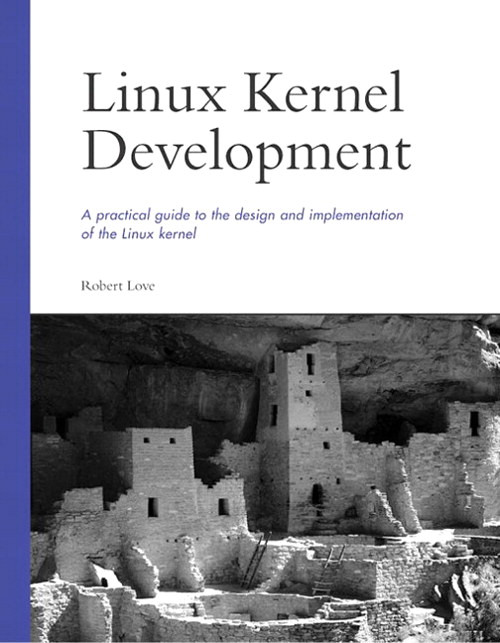
\includegraphics[height=0.4\textheight]{slides/kernel-resources-references/linux-kernel-development.jpg}\\
      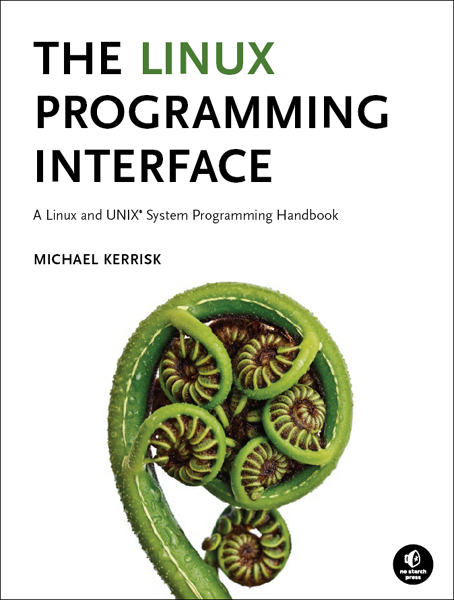
\includegraphics[height=0.4\textheight]{common/linux-programming-interface.png}
    \end{center}
  \end{columns}
\end{frame}

\begin{frame}
  \frametitle{Useful Reading (3)}
  \begin{columns}
    \column{0.7\textwidth}
    Linux Kernel in a Nutshell, Dec. 2006
    \begin{itemize}
    \item By Greg Kroah-Hartman, O'Reilly\\
      \url{http://www.kroah.com/lkn/}
    \item A good reference book and guide on configuring, compiling
      and managing the Linux kernel sources.
    \item Freely available on-line!\\
      Great companion to the printed book for easy electronic searches!\\
      Available as single PDF file on
      \url{https://bootlin.com/community/kernel/lkn/}
    \item Getting old but still containing useful content.
    \end{itemize}
    \column{0.3\textwidth}
    
\includegraphics[width=\textwidth]{slides/kernel-resources-references/linux-kernel-in-a-nutshell.jpg}
  \end{columns}
\end{frame}
